
\documentclass{standalone}

\usepackage{tikz} %Graphics
\usepackage{amsmath}
\usetikzlibrary{shapes.geometric, arrows}


\tikzstyle{startstop} = [ draw=none, minimum width=1.5cm, minimum height=1cm, text centered]
\tikzstyle{process} = [rectangle, rounded corners, minimum width=1.0cm, minimum height=1.0cm, text centered, draw=black, fill=blue!30]
\tikzstyle{process_score} = [circle, minimum width=1.0cm, minimum height=1.0cm, text centered, draw=black, fill=blue!30]

\tikzstyle{arrow} = [thick,->,>=stealth]
\tikzstyle{arrow_back} = [thick,<-,>=stealth]

%\usetikzlibrary{...}
\begin{document}
	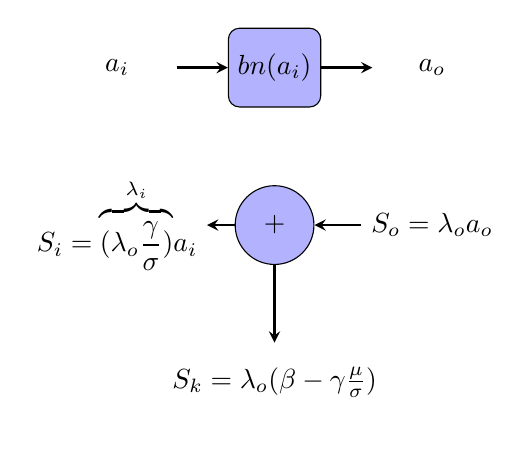
\begin{tikzpicture}[node distance=2cm]
		\node (start) [startstop] {$a_i$};
		\node (af) [process, right of=start] {$bn(a_i)$};
		\node (end) [startstop, right of=af] {$a_o$};
		\draw [arrow] (start) -- (af);
		\draw [arrow] (af) -- (end);
		
		\node (score_in) [startstop, below of=start] {$S_i = \overset{\lambda_i}{\overbrace{(\lambda_o \frac{\gamma}{\sigma})}} a_i$};	
		\node (score_calc) [process_score, right of=score_in] {$+$};
		\node (score_out) [startstop, right of=score_calc] {$S_o = \lambda_o a_o$};	
		\node (score_out_const)[startstop, below of=score_calc] {$S_k = \lambda_o (\beta - \gamma \frac{\mu}{\sigma})$};
		\draw [arrow_back] (score_in) -- (score_calc);
		\draw [arrow_back] (score_calc) -- (score_out);	
		\draw [arrow] (score_calc) -- (score_out_const);	
	\end{tikzpicture}
\end{document}
